\documentclass[../Head/Main.tex]{subfiles}
\begin{document}
	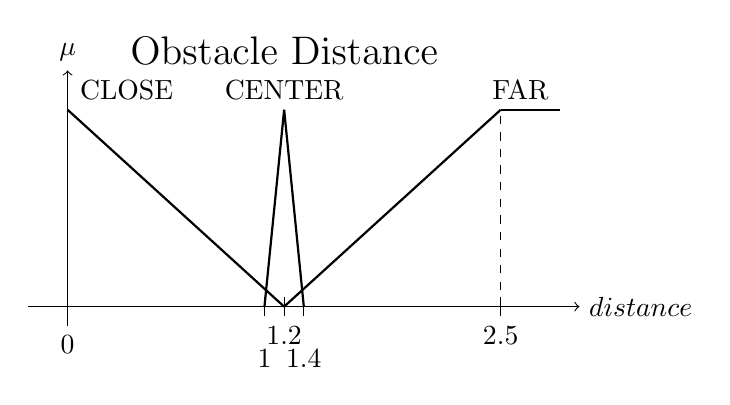
\begin{tikzpicture}
		\draw [->](0,-0.25)--(0,3) node[anchor = south]
			{$\mu$};
		\draw [->](-0.5,0)--(6.5,0) node[right]{$distance$};
		\node[anchor = north] at (0,-0.25) {$0$};
		
		%\node at (3,4.25) {\Large gehge};		
		\node at (2.75,3.25) {\Large Obstacle Distance};
		\node at (0.75,2.75) {CLOSE};
		\node at (5.75,2.75) {FAR};
		\node at (2.75,2.75) {CENTER};	
		
		\draw (2.75,0.125) -- (2.75,-0.125) 
			node[anchor = north] {$1.2$};
			
		\draw (5.5,0.125) -- (5.5,-0.125)
			node[anchor = north] {$2.5$};
		\draw[dashed] (5.5,0) -- (5.5,2.5);
		
		\draw (2.5,0.125) -- (2.5,-0.125) ++(0,-0.3)
			node[anchor = north] {$1$};
			
		\draw (3,0.125) -- (3,-0.125) ++(0,-0.3)
			node[anchor = north] {$1.4$};	
		
		\draw[thick] (5.5,2.5) -- (6.25,2.5);
		
		\draw[thick] (0,2.5) -- (2.75,0);
		\draw[thick] (5.5,2.5) -- (2.75,0);
		
		\draw[thick] (2.5,0) -- (2.75,2.5);
		\draw[thick] (3,0) -- (2.75,2.5);		
	\end{tikzpicture}
\end{document}